\chapter{Gruppenwirkungen auf kubischen Komplexen} % (fold)
\label{cha:3}

\subsection*{Motivation}
\begin{enumerate}[(i)]
	\item Spezieller Fall des Satzes von \textsc{Cartan-Hadamard}: \marginnote{15.01. \\ \ [16]}
	
	Sei $X$ ein vollständiger einfach-zusammenhängender lokaler $\CAT$-Raum.
	Dann ist $X$ $\CAT$. Also:
	
	\[
		\left. \begin{array}{l}
			\text{lokale Eigenschaft: lokal } \CAT \\
			\text{globale Eigenschaft: einfach zusammenhängend}
		\end{array} \right\} \quad \Rightarrow \quad \text{global } \CAT
	\]
	Frage: Wie kann man die lokale $\CAT$-Eigenschaft testen?
	
	Für eine spezielle Klasse von Räumen -- kubische Komplexe -- kann man diese lokale Eigenschaft in eine kombinatorische Eigenschaft übersetzen und somit leichter testen ($\Rightarrow$ \textsc{Gromov}'s Link Condition).
	\item Fragestellung: Wann besitzt die simpliziale Wirkung einer endlich erzeugten Gruppe $G$ auf einen $\CAT$ kubischen Komplex einen Fixpunkt?
	
	Für $\CAT$ kubische Komplexe werden wir eine Methode sehen, um diese Fragestellung anzugehen.
\end{enumerate}

\section{Kubische Komplexe}
\label{sec:3.1}
	Grobe Idee: Wir bauen einen topologischen Raum aus Würfeln.\\
	Als Konvention legen wir fest: $[0,1]^0 = \{0\}$.
	
\begin{definition}[Würfel, Seite]
\label{def:3.1}
	Sei $W:= [0,1]^n \subseteq (\RR^n,d_2)$ ein \Index{Würfel}.
	Eine \Index{Seite} $S \subseteq W$ ist gegeben durch
	\[
		S = S_1 \times \dots \times S_n \text{ mit } S_i \in \{ \{0\}, \{1\}, [0,1]\}.
	\]
	Die eingeschränkte euklidische Metrik auf $W$ bezeichnen wir mit $d_W$.
	Weiter definieren wir die \Index{Dimension} von $W$ wie folgt:
	\[
		\dim(W) := \dim(\sprod{W}) \text{ mit } \sprod{W} \text{ als } \RR\text{-Vektorraum}.
	\]
\end{definition}	
\newpage
\begin{beispiel}
\label{bsp:3.2}
	\mbox{} \\[-1.2cm]
	\begin{figure}[h]
		\centering
		\begin{tikzpicture}[scale=1.5,>=Latex]
			\draw [gray,thick,->] (-.1,0) -- (1.2,0);
			\draw [gray,thick,->] (0,-.1) -- (0,1.2);
			\draw [schraffiert=teal,thick] (0,0) -- (1,0) -- (1,1) -- (0,1) -- cycle;
			
			\draw [color=red,very thick] (0,1) -- (1,1);
			\draw [color=red] (1,0) node[fill,circle,inner sep=1.5pt]{};
			\draw [color=red] (1,1) node[right]{$[0,1] \times \{1\}$};
			\draw [color=red] (1,0) node[below]{$\{1\} \times \{0\}$};
		\end{tikzpicture}
		\caption{Zwei Seiten des Würfels $W = [0,1]^2$.}
	\end{figure}
\end{beispiel}

\begin{definition}[Verklebung, kubischer Komplex]
\label{def:3.3}
	Seien $W_1,W_2$ zwei Würfel und $S_1 \subseteq W_1$ und $S_2 \subseteq W_2$ Seiten.
	Eine Isometrie $\varphi \colon S_1 \rightarrow S_2$ heißt \Index{Verklebung} von $W_1$ und $W_2$.
	Sei nun $\mathcal{W}$ eine Familie von Würfeln und $\mathcal{V}$ eine Familie von Verklebungen von Würfeln aus $\mathcal{W}$ mit folgenden Eigenschaften:
	\begin{enumerate}[(i)]
		\item Kein Würfel ist mit sich selbst verklebt.
		\item Je zwei Würfel aus $\mathcal{W}$ sind höchstens einmal miteinander verklebt.
	\end{enumerate}
	Sei $\sim$ die durch
	\[
		x \sim y \quad :\Leftrightarrow \quad \text{es existiert ein } \varphi \in \mathcal{V} \text{ mit } x \in \dom(\varphi) \text{ und } \varphi(x) = y
	\]
	erzeugte Äquivalenzrelation auf $\bigsqcup_{W \in \mathcal{W}} W$. Die Menge
	\[
		X := \enbrace*{ \bigsqcup_{W \in \mathcal{W}} W}\diagup\sim
	\]
	heißt kubischer Komplex definiert durch $(\mathcal{W},\mathcal{V})$.
	Die Dimension von $X$ ist definiert durch
	\[
		\dim(X) := \sup\{ \dim(W) : W \in \mathcal{W}\}.
	\]
\end{definition}

\begin{beispiel}
\label{bsp:3.4}
	\mbox{} \\[-1.4cm]
	\begin{align*}
		\mathcal{W} := \ &\{W_1 = [0,1]^2, W_2 = [0,1]^2, W_3 = [0,1]\} \\
		\mathcal{V} := \ &\{\varphi_1 \colon \{0\} \times \{0\} \subseteq W_1 \rightarrow \{1\} \times \{1\} \subseteq W_2, \varphi_2 \colon [0,1] \times \{1\} \subseteq W_2 \rightarrow [0,1] = W_3\}
	\end{align*}
\end{beispiel}

\begin{figure}[h]
	\centering
	\begin{tikzpicture}[scale=1,>=Latex]
		\draw [thick,schraffiert=teal] (0,0) -- (1,0) -- (1,1) -- (0,1) -- cycle;
		\draw [thick,schraffiert=teal] (2,0) -- (3,0) -- (3,1) -- (2,1) -- cycle;
		\draw [very thick,color=red] (4,0) -- (5,0);
		\draw [very thick,color=red] (2,1) -- (3,1);
		
		\draw (.5,0) node[below]{$W_1$};
		\draw (2.5,0) node[below]{$W_2$};
		\draw (4.5,0) node[below]{$W_3$};
		
		\draw [color=Green4,->] (0,0) .. controls (-1,1) and (1,2.5) ..   (3,1);
		\draw [color=Green4,->] (2.5,1) to[out=90,in=90] (4.5,0);
		
		\draw [color=RoyalBlue2] (0,0) node[fill,circle,inner sep=2pt]{};
		\draw [color=RoyalBlue2] (3,1) node[fill,circle,inner sep=2pt]{};
		\draw [color=Green4] (4,1) node[right]{$\varphi_2$};
		\draw [color=Green4] (1,1.6) node[above]{$\varphi_1$};
	\end{tikzpicture} \hspace{1.5cm}
	\begin{tikzpicture}[scale=1,>=Latex]
		\draw (0,1.8) node[right]{$\mathbf{X}$};
		\draw [thick,schraffiert=teal] (0,0) -- (1,0) -- (1,1) -- (0,1) -- cycle;
		\draw [thick,schraffiert=teal] (1,1) -- (2,1) -- (2,2) -- (1,2) -- cycle;
		\draw [very thick,red] (0,1) -- (1,1);
		\draw [color=RoyalBlue2] (1,1) node[fill,circle,inner sep=2pt]{};
	\end{tikzpicture}
\end{figure}
\newpage
\begin{definition}
\label{def:3.5}
	Seien $x,y \in X$ beliebig.
	Ein Weg $c$ von $x$ nach $y$ in $X$ ist definiert als eine endliche Folge $c=(x_0,\dots,x_m), x_i \in X$ mit $x_0 = x$, $x_m = y$ und folgender Eigenschaft:
	Für alle $i \in \{0,\dots,m-1\}$ existiert ein Würfel $W_i \in \mathcal{W}$ mit $x_i,x_{i+1} \in W_i$.
	
	Weiter definieren wir die Länge von $c$ als
	\[
		\ell(c) = \ell((x_0,\dots,x_m)) = \sum\limits_{i=0}^{m-1} d_{W_i} (x_i,x_{i+1}).
	\]
	$X$ heißt \textbf{wegzusammenhängend}, wenn es für je zwei Elemente aus $X$ ein solcher Weg existiert. \index{zusammenhängend!wegzusammenhängend}
	
	Nun definieren wir auf $X$ wegzusammenhängend eine Metrik:
	\begin{align*}
		d_X \colon X \times X &\longrightarrow \RR_{\geq 0} \\
		(x,y) &\longmapsto \inf\{ \ell(c) : c \text{ ist ein Weg von } x \text{ nach } y\}
	\end{align*}
\end{definition}

Ab jetzt betrachten wir einen wegzusammenhängenden kubischen Komplex immer mit der Metrik $d_X$.

\begin{beispiel}
\label{bsp:3.6}
	$c=(x,x_1,x_2,y)$ ist ein Weg von $x$ nach $y$.
	\begin{figure}[h]
		\centering
		\begin{tikzpicture}[scale=1,>=Latex]
			\draw [thick] (.5,3) node[fill,circle,inner sep=1.5pt]{}
			-- (1.5,2.5) node[fill,circle,inner sep=1.5pt]{}
			-- (2.4,3.5) node[fill,circle,inner sep=1.5pt]{}
			-- (1.5,2.5)
			to[pos=.6] coordinate (X) (2,1.5) node[fill,circle,inner sep=1.5pt,color=RoyalBlue2]{}
			-- (1,1) node[fill,circle,inner sep=1.5pt]{}
			-- (2,1.5)
			-- (3.5,1) node[fill,circle,inner sep=1.5pt,color=RoyalBlue2]{}
			-- (3,0) node[fill,circle,inner sep=1.5pt]{}
			-- (3.5,1)
			to[pos=.6] coordinate (Y) (4.5,.25) node[fill,circle,inner sep=1.5pt]{};
			
			\draw [very thick,color=RoyalBlue2] (X) -- (2,1.5) -- (3.5,1) -- (Y);
			\draw [color=RoyalBlue2] (X) node[left]{$x$};
			\draw [color=RoyalBlue2] (2,1.5) node[anchor=south west]{$x_1$};
			\draw [color=RoyalBlue2] (3.5,1) node[above]{$x_2$};
			\draw [color=RoyalBlue2] (Y) node[anchor=south west]{$y$};
			\draw (X) node[fill,circle,inner sep=1.5pt,color=RoyalBlue2]{};
			\draw (Y) node[fill,circle,inner sep=1.5pt,color=RoyalBlue2]{};
		\end{tikzpicture}
	\end{figure}
\end{beispiel}

\subsection{Simpliziale Bäume}
\label{subsec:3.1.1}

Erinnerung:
Sei $\Gamma = (V,E)$ ein ungerichteter Graph.
$\Gamma$ heißt \textbf{(simplizialer) Baum}, wenn $\Gamma$ wegzusammenhängend ist und $\Gamma$ keine Kreise hat. \index{Baum}

Bäume haben eine natürliche Struktur als $1$-dimensionale kubische Komplexe.
Wir betrachten nun Bäume mit dieser kubischen Struktur.

\begin{satz}
\label{satz:3.7}
	Bäume sind vollständige $\CAT$-Räume. (\autoref{aufg:7.3})
\end{satz}

Fragestellung:
Sei $G$ eine endlich erzeugte Gruppe und $\Phi\colon G \rightarrow \Isom(X)$ eine isometrische Wirkung auf einem Baum. \marginnote{20.01. \\ \ [17]}
Hat $\Phi$ einen globalen Fixpunkt, das heißt existiert ein $x \in X$, sodass für alle $g \in G$ gilt: $\Phi(g)(x)=x$?

Wir betrachten simpliziale Wirkungen, das heißt
\[
	\Phi(G) \subseteq \SIsom(X) := \{f\colon X \rightarrow X : f \text{ ist Isometrie und } f(\text{Ecke}) = \text{ Ecke' für alle Ecken in } X\}
\]
Dies ist tatsächlich eine Einschränkung: Für den Baum $X=\RR$ ist $f\colon X \rightarrow X, x \mapsto x + \frac{1}{2}$ eine Isometrie, aber keine simpliziale Isometrie.

Wir schränken das Bild von $\Phi$ noch ein wenig ein:
Wir betrachten nur simpliziale Isometrien ohne Inversionen.
Eine simpliziale Isometrie $f \colon X \rightarrow X$ hat eine Inversion, wenn folgendes passiert: \begin{figure}[h]
	\centering
	\begin{tikzpicture}[scale=1.5,>=Latex]
		\draw [ultra thick] (0,0) node[below]{$v_1$} -- (1.7,0) node[below]{$v_2$};
		\draw (0,0) node[fill,circle,inner sep=2pt]{};
		\draw (1.7,0) node[fill,circle,inner sep=2pt]{};
		
		\draw [->,thick] (2.2,0) to [bend angle=30,bend left] coordinate[pos=.5] (A) (3.8,0);
		\draw (A) node[above]{$f$};
		
		\draw [ultra thick] (4.3,0) node[below]{$v_2$} -- (6,0) node[below]{$v_1$};
		\draw (4.3,0) node[fill,circle,inner sep=2pt]{};
		\draw (6,0) node[fill,circle,inner sep=2pt]{};
	\end{tikzpicture}
\end{figure}

Eine Methode, um die Frage zu beantworten, ist das Theorem von \textsc{Helly} für simpliziale Bäume.

\begin{no-satz}[\textsc{Helly}, 1923]
	Sei $\mathcal{S} := \{S_1, \dots, S_l : S_i \subseteq \RR^d, S_i \neq \emptyset, S_i \text{ ist abgeschlossen und konvex für } i = 1, \dots, l\}$ eine endliche Familie.
	Wenn sich jeweils $(d+1)$ Elemente aus $\mathcal{S}$ nichttrivial schneiden, dann ist $\cap \mathcal{S}$ nichtleer.
\end{no-satz}

\begin{no-bem}
	$d+1$ ist eine minimale Schranke, denn zum Beispiel im $\RR^2$ ist $S_1 \cap S_2, S_2 \cap S_3, S_1 \cap S_3 \neq \emptyset$ und $S_1 \cap S_2 \cap S_3 = \emptyset$ möglich.
	
	\begin{figure}[h]
		\centering
		\begin{tikzpicture}[scale=.5,>=Latex]
			\draw [->,very thick] (-1,0) -- (4.5,0);
			\draw [->,very thick] (0,-1) -- (0,3.5);
			
			\draw (-.8,2) -- (4,2) node[right]{$S_3$};
			\draw (-1,2.5) -- (2.5,-1) node[right]{$S_2$};
			\draw (-.5,-1) -- (3.5,3) node[right]{$S_1$};
		\end{tikzpicture}
	\end{figure}
\end{no-bem}

Gibt es eine Verallgemeinerung des Theorems für $\CAT$-Räume?
Ja, zum Beispiel für Bäume:

\begin{no-satz}[\textsc{Helly}s Theorem für Bäume]
	Sei $X$ ein Baum und $\mathcal{S} = \{S_1,\dots,S_l\}$ eine endliche Familie von Teilbäumen.
	Wenn sich jeweils zwei Elemente aus $\mathcal{S}$ nichttrivial schneiden, dann ist $\cap \mathcal{S}$ nicht leer. (\autoref{aufg:7.2})
\end{no-satz}

\begin{satz}
\label{satz:3.8}
	Sei $G = \sprod{g_1,\dots,g_k}$ eine endlich erzeugte Gruppe.
	Sei $X$ ein Baum und $\Phi\colon G \rightarrow \SIsom(X)$ eine simpliziale Wirkung ohne Inversionen.
	Wenn $\Fix_\Phi(\sprod{g_i}) \neq \emptyset$ und $\Fix_\Phi(\sprod{g_i}) \cap \Fix_\Phi(\sprod{g_j}) \neq \emptyset$ für alle $i,j \in \{1,\dots,k\}$, dann gilt $\Fix_\Phi(G) \neq \emptyset$.
\end{satz}

\begin{beweis}
	$\Fix_\Phi(\sprod{g_i}) \subseteq X$ ist ein Teilbaum von $X$.
	Mit \textsc{Helly}s Theorem für Bäume folgt $\emptyset \neq \cap \Fix_\Phi(\sprod{g_i}) = \Fix_\Phi(\sprod{g_1,\dots,g_k}) = \Fix_\Phi(G)$. \qedhere
\end{beweis}

\begin{satz}[Verallgemeinerung]
\label{satz:3.9}
	Sei $G = \sprod{g_1,\dots,g_k}$ eine endlich erzeugte Gruppe und $X$ ein Baum.
	Sei $\Phi\colon G \rightarrow \Isom(X)$ eine isometrische Wirkung.
	Wenn $\Fix_\Phi(\sprod{g_i}) \neq \emptyset$ und $\Fix_\Phi(\sprod{g_i}) \cap \Fix_\Phi(\sprod{g_j}) \neq \emptyset$ für alle $i,j \in \{1,\dots,k\}$, dann ist $\Fix_\Phi(G) \neq \emptyset$. \autoref{aufg:7.2}
\end{satz}

\begin{no-bsp}
\label{bsp:3.10}
	Für $n \geq 3$ sei $F_n = \sprod{x_1, \dots, x_n}$ die freie Gruppe vom Rang $n$ und $\Aut(F_n)$ der Automorphismengruppe von $F_n$. \index{Automorphismus}
	Für zwei Automorphismen $\alpha, \beta \in \Aut(F_n)$ ist $\alpha \beta := \beta \circ \alpha$.
	Wir definieren \textbf{Rechtsnielsenautomorphismen} für $i,j \in \{1, \dots, n\}, i \neq j$.
	\begin{align*}
		\rho_{i,j} \colon F_n &\longrightarrow F_n \\
		x_k &\longmapsto \begin{cases}
			x_ix_j, & \text{falls } k=i \\
			x_k, & \text{falls } k \neq i
		\end{cases}
	\end{align*}
	Weiter definieren wir die Involution
	\begin{align*}
		(x_i,x_j)\colon F_n &\longrightarrow F_n \\
			s_k &\longmapsto \begin{cases}
				x_j, & \text{falls } k=i \\
				x_i, & \text{falls } k=j \\
				x_k, & \text{sonst}
			\end{cases}
	\end{align*}
	und
	\begin{align*}
		e_i \colon F_n &\longrightarrow F_n \\
		x_k &\longmapsto \begin{cases}
			x_i^{-1}, & \text{falls } k = i \\
			x_k, &\text{falls } k \neq i.
		\end{cases}
	\end{align*}
	Es gilt $\rho_{i,j}, (x_i,x_j), e_i \in \Aut(F_n)$, und es ist
	\[
		\Aut(F_n) = \sprod{\Underbrace{(x_1,x_2)e_1e_2, (x_2,x_3)e_1, (x_i,x_{i+1}), e_2\rho_{1,2},e_n : i = 3, \dots n-1}{=:Y}}
	\]
	Es ist $\ord(\alpha) = 2$ für $\alpha \in Y$ und $\abs{\sprod{\alpha,\beta}} < \infty$ für $\alpha,\beta \in Y$.
	
	Sei nun $X$ ein Baum und $\Phi\colon \Aut(F_n) \rightarrow \Isom(X)$ eine isometrische Wirkung.
	Dann ist $\Fix_\Phi(\Aut(F_n)) \neq \emptyset$, denn:
	\begin{itemize}
		\item Nach \textsc{Bruhat-Tits} (\autoref{BTFT}) ist $\Fix_\Phi(\sprod{\alpha}) \neq \emptyset$, da Bäume $\CAT$ und vollständig sind.
		\item Ebenso ist $\Fix_\Phi(\sprod{\alpha}) \cap \Fix_\Phi(\sprod{\beta}) \neq \emptyset$ für $\alpha, \beta \in Y$ beliebig.
		\item Mit \autoref{satz:3.9} folgt somit $\Fix_\Phi(\Aut(F_n)) \neq \emptyset$.
	\end{itemize}
\end{no-bsp}

\begin{definition}[Eigenschaft $\prF{X}$]
\label{def:3.10}
	Sei  $\mathcal{X}$ eine Klasse von metrischen Räumen. \index{Eigenschaft $\prF{X}$}
	Eine Gruppe $G$ hat die Eigenschaft $\prF{X}$, wenn jede isometrische Wirkung auf jedem Raum aus $\mathcal{X}$ einen globalen Fixpunkt hat.
\end{definition}

\begin{beispiel}[\textsc{Bogopolski}, 1973]
\label{bsp:3.11}
	Sei $\mathcal{A}$ die Klasse der Bäume.
	Für $n \geq 3$ hat $\Aut(F_n)$ die Eigenschaft $\prF{A}$. 
\end{beispiel}

Frage:
Sei $G \leq \Aut(F_n), n \geq 3$ eine Untergruppe mit $[\Aut(F_n) : G] < \infty$.
Hat $G$ die Eigenschaft $\text{F}\mathcal{A}$?
Für $n = 3$ lautet die Antwort nein, für $n \geq 4$ ist die Frage bislang ungeklärt.

Eine Anwendung der Eigenschaft $\prF{A}$ ist die Strukturtheorie:
Sei $G$ eine endlich erzeugte Gruppe.
Kann man $G$ in \enquote{einfache} Bestandteile zerlegen?
\begin{itemize}
	\item Zum Beispiel in ein kartesisches Produkt $G \simeq G_1 \times G_2$.
	\item Zum Beispiel in ein amalgamiertes Produkt $G \simeq G_1 *_H G_2$.
\end{itemize}

\begin{no-satz}[\textsc{Serre}]
	Sei $G$ eine endlich erzeugte Gruppe.
	Wenn $G$ die Eigenschaft $\text{F}\mathcal{A}$ hat, dann ist $G$ kein nichttriviales amalgamiertes Produkt.
\end{no-satz}

Im Seminar im Sommersemester 2016 werden wir sehen, dass $\Aut(F_n)$ für $n \geq 3$ kein nichttriviales amalgamiertes Produkt ist.

\subsection{\textsc{Helly}s Theorem für CAT(0) kubische Komplexe}
\label{subsec:3.1.2}

\begin{definition}
\label{def:3.12}
	Sei $X$ ein kubischer Komplex definiert durch $(\mathcal{W},\mathcal{V})$.
	Eine Teilmenge $Y \subseteq X$ heißt \textbf{kubischer Unterkomplex}, wenn es eine Teilfamilie $\mathcal{W'} \subseteq \mathcal{W}$ existiert, sodass
	\[
		Y = \bigsqcup_{W \in \mathcal{W}'} W \diagup \sim.
	\]
	Dabei ist $\sim$ erzeugt durch
	\[
		x \sim y \quad :\Leftrightarrow \quad \text{es existiert ein } \varphi \colon S_1 \rightarrow S_2 \in \mathcal{V} \text{ mit } S_1,S_2 \text{ sind Seiten von } W_1,W_2 \in \mathcal{W'} \text{ und } \varphi(x) = y
	\]
\end{definition}

\begin{bemerkung}
\label{bem:3.13}
	Wir setzen nicht voraus, dass kubische Unterkomplexe wegzusammenhängend sind.
	\begin{figure}[h]
		\centering
		\begin{tikzpicture}[scale=.8,>=Latex]
			\draw (0,2.5) node[right]{$\mathbf{X}$};
			\draw [very thick] (2,0) -- (1,0) -- (1,1) -- (0,1) -- (0,2) -- (1,2) -- (1,1) -- (2,1) -- (2,2) -- (1,2) -- (1.5,2.5) -- (2.5,2.5) -- (2,2);
			\draw [thick] (2.5,2.5) -- (2.5,1.5) -- (2,1) -- (2,0) -- (3,0);
			
			\draw (6,2.5) node[right]{$\mathbf{Y}$};
			\draw [very thick] (6,1) -- (7,1) -- (7,2) -- (6,2) -- cycle;
			\draw [very thick] (8,0) -- (9,0);
		\end{tikzpicture}
	\end{figure}
\end{bemerkung}
\newpage
\begin{theorem}[\textsc{Helly}s Theorem für $\CAT$ kubische Komplexe]
\label{thm:3.14}
	Sei $X$ ein $\CAT$ kubischer Komplex und $\mathcal{S}$ eine endliche Familie von nichtleeren konvexen kubischen Unterkomplexen.
	Wenn der Schnitt von jeweils zwei Elementen aus $\mathcal{S}$ nicht leer ist, dann ist $\cap \mathcal{S}$ nicht leer.
\end{theorem}

Um dies zu beweisen, müssen wir zuerst Hyperebenen einführen.

\begin{definition}[Quadratäquivalenz]
	\label{def:3.15}
	Sei $X$ ein kubischer Komplex. \marginnote{27.01. \\ \ [18]}
	Wir definieren
	\[
		\mathcal{K} := \{ k \subseteq X : k \text{ ist isometrisch zu } [0,1] \text{ und es ex. ein } W \in \mathcal{W} \text{, sodass } k \text{ eine Seite von } W \text{ ist}\}.
	\]
	$\mathcal{K}$ ist also die Menge aller Kanten von $X$.
	Wir definieren wie folgt eine Äquivalenz auf $\mathcal{K}$:
	\[
		k \approx k' \quad :\Leftrightarrow \quad k \text{ liegt gegenüber von } k' \text{ in einem zweidimensionalen Würfel von } X.
	\]
	Das ist aber noch keine Äquivalenzrelation, da $k \not\approx k.$
	
	Sei nun $\sim$ die von $\approx$ erzeugte Äquivalenzrelation.
	Wenn $k \sim k'$, dann sagen wir: $k$ und $k'$ sind \Index{quadratäquivalent}.
	
	\begin{figure}[h]
		\centering
		\begin{tikzpicture}[scale=1,>=Latex]
			\draw [ultra thick,dashed, color=red] (1.5,1.5) -- (1.5,2.5);
			\draw [dashed] (1,1) -- (1.5,1.5) -- (2.5,1.5);
			\draw (0,1) -- (1,1) -- (2,1) -- (2,0) -- (1,0);
			\draw (2,1) -- (2.5,1.5) -- (3.5,1.5);
			\draw (3.5,2.5) -- (2.5,2.5) -- (1.5,2.5) -- (1,2) -- (2,2) -- (2.5,2.5);
			
			\draw [very thick,color=red] (0,1) -- (0,2);
			\draw [very thick,color=red] (1,1) -- (1,2);
			\draw [very thick,color=red] (2,1) -- (2,2);
			\draw [very thick,color=red] (2.5,1.5) -- (2.5,2.5);
			\draw [very thick,color=red] (3.5,1.5) -- (3.5,2.5);
			\draw [color=red] (0,1.5) node[left]{$k$};
			
			\draw [very thick,color=teal] (1,0) -- (1,1);
			\draw [very thick,color=teal] (0,2) -- (1,2);
			\draw [color=teal] (1,0.5) node[left]{$e_2$};
			\draw [color=teal] (0.5,2) node[above]{$e_1$};			
		\end{tikzpicture}
		\caption{Die rot markierten Kanten sind alle zu $k$ quadratäquivalenten Kanten. $e_1$ und $e_2$ sind nicht quadratäquivalent zu $k$.}
	\end{figure}
\end{definition}

\begin{definition}[Mittelwürfel, transversal, Hyperebene]
	\label{def:3.16}
	Sei $W = [0,1]^n \in \mathcal{W}$ ein Würfel.
	Für $i = 1, \dots, n$ definieren wir den \Index{Mittelwürfel} 
	\[
		W_i := [0,1]^{i-1} \times \penbrace*{\frac{1}{2}} \times [0,1]^{n-i}
	\]
	\mbox{} \\[-1cm]
	
	\begin{figure}[h]
		\centering
		\begin{tikzpicture}[scale=1.5,>=Latex]
			\draw [->,very thick] (0,0) -- (0,1.4) node[right] {$x_3$};
			\draw [->,very thick] (0,0) -- (1.4,0) node[right] {$x_1$};
			\draw [->,very thick] (0,0) -- (-.7,-.7) node[left] {$x_2$};
			
			\draw (-.5,-.5) -- (-.5,.5) -- (0,1) -- (0,0) -- (-.5,-.5);
			\draw (.5,-.5) -- (.5, .5) -- (1,1) -- (1,0) -- (.5,-.5);
			\draw (-.5,.5) -- (.5,.5) -- (1,1) -- (0,1) -- (-.5,.5);
			\draw (-.5,-.5) -- (.5,-.5);
		
			\draw [color=teal,schraffiert=teal] (0,-.5) -- (.5,0) -- (.5,1) -- (0,.5) -- (0,-.5);
			\draw [color=teal] (0,-.5) node[below]{$W_1$};
		
			\draw [color=red,schraffiert=red] (-.25,-.25) -- (.75,-.25) -- (.75,.75) -- (-.25,.75) -- (-.25,-.25);
			\draw [color=red] (-.4,.85) node{$W_2$};
		
			\draw [color=blue,schraffiert=blue] (-.5,0) -- (.5,0) -- (1,.5) -- (0,.5) -- (-.5,0);
			\draw [color=blue] (1.0,.5) node[right]{$W_3$};
		\end{tikzpicture}
	\end{figure}
	
	Sei $k \in \mathcal{K}$ eine beliebige Kante.
	Ein Mittelwürfel $W_i$ heißt \Index{transversal} zu $k$, wenn gilt
	\[
		W_i \cap \mathcal{K} = \{ \text{Mittelpunkte von } k' : k' \in [k]\}.
	\]
	Wir schreiben $W_i \pitchfork k$.
	Die Menge aller zu $k$ transversalen Mittelwürfel bezeichnen wir mit $k^\pitchfork$.
	Die \Index{Hyperebene} zu $k$ ist dann definiert durch
	\[
		H(k) := \bigcup_{W_i \in k^\pitchfork} W_i
	\]
	
	\begin{figure}[h]
		\centering
			\begin{tikzpicture}[scale=1.25]
			\draw (2,2) -- (1,2) -- (1,1) -- (2,1) -- (2,0) -- (1,0) -- (1,1) -- (0,1) -- (0,2) -- (1,2) -- (1.5,2.5) -- (3.5,2.5) -- (3.5,1.5) -- (2.5,1.5) -- (2,1) -- (2,2) -- (2.5,2.5) -- (2.5,1.5);
			\draw [color=red,very thick] (2,2) -- (2,1);
			\draw [color=red,very thick] (1,1) -- (1,2);
			\draw [color=red,very thick] (2.5,2.5) -- (2.5,1.5);

			\draw [color=red,very thick] (0,1) -- (0,2);
			\draw [color=red,very thick] (3.5,2.5) -- (3.5,1.5);
			\draw [dashed] (1,1) -- (1.5,1.5);
			\draw [dashed] (1.5,1.5) -- (2.5,1.5);
			\draw [color=red,ultra thick,dashed] (1.5,2.5) -- (1.5,1.5);
			\draw [color=red] (2,1) node[anchor=north west] {$[k]$};
			
			\draw [color=blue,very thick] (0,1.5) -- (1,1.5);
			\draw [color=blue,schraffiert=blue,very thick] (1,1.5) -- (2,1.5) -- (2.5,2) -- (1.5,2) -- (1,1.5);
			\draw [color=blue,very thick] (2.5,2) -- (3.5,2);
			\draw [color=blue] (3,2) node[below] {$H(k)$};
			\draw [color=red] (0,1.5) node[left]{$k$};
			\end{tikzpicture}
	\end{figure}
\end{definition}

\begin{beispiel}
	\label{bsp:3.17}
	In einem Baum sind Mittelwürfel gerade die Mittelpunkte der Kanten.
	Da in einem Baum keine zweidimensionalen Würfel existieren, gibt es zu einer Kante $k$ keine weiteren quadratäquivalenten Kanten.
	Demzufolge ist der Mittelpunkt von $k$ die Hyperebene zu $k$.
	
	In kubischen Komplexen, die nicht $\CAT$ sind, können Hyperebenen sich selbst schneiden.
	
	\mbox{} \\[-4cm]
	\begin{figure}[h]
		\centering
		\begin{tikzpicture}[scale=1.7,>=Latex]
			\draw [very thick] (0,0) -- (.5,.5) -- (1,0);
			\draw [very thick,color=red] (1,0) -- (2,0);
			\draw [very thick] (0,1) -- (.5,.5) -- (1,1) -- (1,2);
			\draw [very thick] (1,1) -- (2,1);
						
			\draw [very thick] (2,0) -- (2.5,0.5);
			\draw [very thick] (2,0) -- (2.5,-0.5);
						
			\draw (0,0) node[fill,circle,inner sep=1.5pt]{};
			\draw (.5,.5) node[fill,circle,inner sep=1.5pt]{};
			\draw (0,1) node[fill,circle,inner sep=1.5pt]{};
			\draw (1,1) node[fill,circle,inner sep=1.5pt]{};
			\draw (1,2) node[fill,circle,inner sep=1.5pt]{};
			\draw (2,1) node[fill,circle,inner sep=1.5pt]{};
			\draw (1,0) node[fill,circle,inner sep=1.5pt]{};
			\draw (2,0) node[fill,circle,inner sep=1.5pt]{};
			\draw (2.5,-.5) node[fill,circle,inner sep=1.5pt]{};
			\draw (2.5,.5) node[fill,circle,inner sep=1.5pt]{};
			
			\draw [color=blue] (1.5,0) node[fill,circle,inner sep=1.5pt]{};
			\draw [color=blue] (1.5,0.1) node[above]{$H(k)$};
			\draw [color=red] (1.5,-.1) node[below]{$k$};
		\end{tikzpicture}~\hspace{5cm}~
		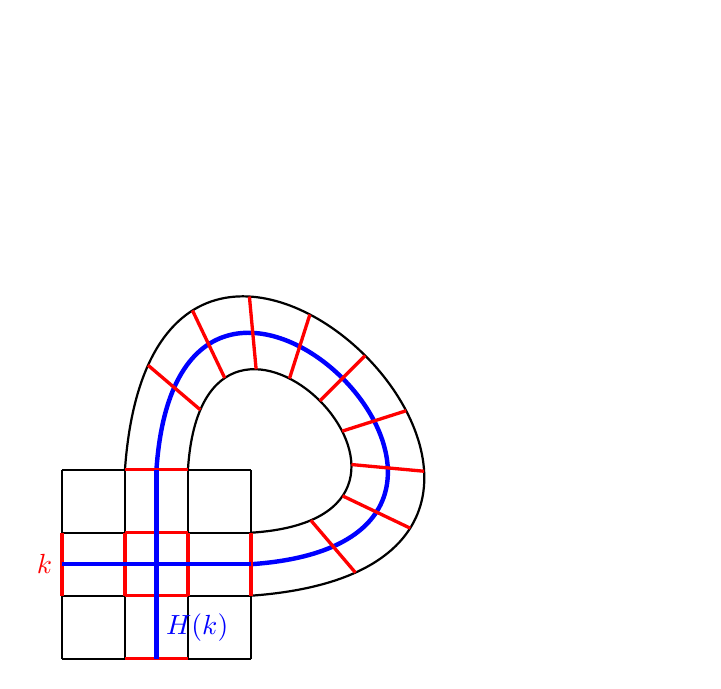
\begin{tikzpicture}[scale=.8]
			\draw [thick,step=1] (0,0) grid (3,3);
			
			\draw [thick] (1,3) .. controls (1.5,10) and (10,1.5) .. 
				coordinate[pos=.1] (A1)
				coordinate[pos=.2] (A2)
				coordinate[pos=.3] (A3)
				coordinate[pos=.4] (A4)
				coordinate[pos=.5] (A5)
				coordinate[pos=.6] (A6)
				coordinate[pos=.7] (A7)
				coordinate[pos=.8] (A8)
				coordinate[pos=.9] (A9)
				(3,1);
			\draw [thick] (2,3) .. controls (2.25,7) and (7,2.25) .. 
				coordinate[pos=.1] (B1)
				coordinate[pos=.2] (B2)
				coordinate[pos=.3] (B3)
				coordinate[pos=.4] (B4)
				coordinate[pos=.5] (B5)
				coordinate[pos=.6] (B6)
				coordinate[pos=.7] (B7)
				coordinate[pos=.8] (B8)
				coordinate[pos=.9] (B9)
				(3,2);
			
			\draw [ultra thick,color=blue] (1.5,3) .. controls (1.875,8.5) and (8.5,1.875) .. (3,1.5);
			
			\foreach \x in {1,...,9} {
				\draw [very thick,color=red] (A\x) -- (B\x);
			};
			
			\draw [very thick,color=red] (0,1) -- (0,2);
			\draw [very thick,color=red] (1,1) -- (1,2);
			\draw [very thick,color=red] (2,1) -- (2,2);
			\draw [very thick,color=red] (3,1) -- (3,2);
			
			\draw [very thick,color=red] (1,0) -- (2,0);
			\draw [very thick,color=red] (1,1) -- (2,1);
			\draw [very thick,color=red] (1,2) -- (2,2);
			\draw [very thick,color=red] (1,3) -- (2,3);
			
			\draw [ultra thick,color=blue] (0,1.5) -- (3,1.5);
			\draw [ultra thick,color=blue] (1.5,0) -- (1.5,3);
			
			\draw [color=red] (0,1.5) node[left]{$k$};
			\draw [color=blue] (1.5,0.5) node[right]{$H(k)$};
		\end{tikzpicture}
	\end{figure}
\end{beispiel}

\begin{satz}[{\cite{Sageev}}]
	\label{satz:3.18}
		Sei $X$ ein $\CAT$ kubischer Komplex und $H$ eine beliebige Hyperebene.
		Dann besitzt $X \setminus H$ genau zwei Zusammenhangskomponenten, also
		\[
			\# \pi_0(X \setminus H) = 2.
		\]
		Wir schreiben $X - H = H^+ \sqcup H^-$ mit $H^+, H^- \in \pi_0(X \setminus H)$ und nennen $H^+,H^-$ \textbf{Halbräume} in $X$. \index{Halbraum}
\end{satz}
\begin{figure}[h]
	\centering
	\begin{tabular}{ccc}
		\begin{tikzpicture}
		\draw [color=purple,schraffiert=purple] (0,1) -- (.5,1) -- (.5,2) -- (0,2) -- (0,1);
		\draw [color=teal,schraffiert=teal] (.5,1) -- (.5,2) -- (1,2) -- (1.5,2.5) -- (3.5,2.5) -- (3.5,1.5) -- (2.5,1.5) -- (2,1) -- (2,0) -- (1,0) -- (1,1) -- (.5,1);
		\draw [color=blue,ultra thick] (.5,1) -- (.5,2);
		
		\draw [thick] (2,2) -- (0,2) -- (0,1) -- (2,1) -- (2,0) -- (1,0) -- (1,2) -- (1.5,2.5) -- (3.5,2.5) -- (3.5,1.5) -- (2.5,1.5) -- (2,1) -- (2,2) -- (2.5,2.5) -- (2.5,1.5);
		
		\draw [color=teal] (3.55,2) node[right] {$H^+$};
		\draw [color=purple] (.25,1) node[below] {$H^-$};
		\draw [color=blue] (.5,2) node[above] {$H$};
		\end{tikzpicture}
		&
		\begin{tikzpicture}
		\draw [color=purple,schraffiert=purple] (1.5,0) -- (1,0) -- (1,1) -- (0,1) -- (0,2) -- (1,2) -- (1.5,2.5) -- (2,2.5) -- (1.5,2) -- (1.5,0);
		\draw [color=teal,schraffiert=teal] (1.5,0) -- (1.5,2) -- (2,2.5) -- (3.5,2.5) -- (3.5,1.5) -- (2.5,1.5) -- (2,1) -- (2,0) -- (1.5,0);
		\draw [color=blue,ultra thick] (2,2.5) -- (1.5,2) -- (1.5,0);
		
		\draw [thick] (2,2) -- (0,2) -- (0,1) -- (2,1) -- (2,0) -- (1,0) -- (1,2) -- (1.5,2.5) -- (3.5,2.5) -- (3.5,1.5) -- (2.5,1.5) -- (2,1) -- (2,2) -- (2.5,2.5) -- (2.5,1.5);
		
		\draw [color=teal] (2.1,1) node[right] {$H^+$};
		\draw [color=purple] (.25,1) node[below] {$H^-$};
		\draw [color=blue] (2,2.5) node[above]{$H$};
		\end{tikzpicture}
		&
		\begin{tikzpicture}
		\draw [color=purple,schraffiert=purple] (3,2.5) -- (3,1.5) -- (2.5,1.5) -- (2,1) -- (2,0) -- (1,0) -- (1,1) -- (0,1) -- (0,2) -- (1,2) -- (1.5,2.5) -- (3,2.5);
		\draw [color=teal,schraffiert=teal] (3,2.5) -- (3.5,2.5) -- (3.5,1.5) -- (3,1.5) -- (3,2.5);
		\draw [color=blue,ultra thick] (3,2.5) -- (3,1.5);
		
		\draw [thick] (2,2) -- (0,2) -- (0,1) -- (2,1) -- (2,0) -- (1,0) -- (1,2) -- (1.5,2.5) -- (3.5,2.5) -- (3.5,1.5) -- (2.5,1.5) -- (2,1) -- (2,2) -- (2.5,2.5) -- (2.5,1.5);
		
		\draw [color=teal] (3.55,2) node[right] {$H^+$};
		\draw [color=purple] (.5,1) node[below]{$H^-$};
		\draw [color=blue] (3,1.5) node[below]{$H$};
		\end{tikzpicture}
		\\
		\begin{tikzpicture}
		\draw [color=teal,schraffiert = teal] (0,1.5) -- (0,2) -- (1,2) -- (1.5,2.5) -- (3.5,2.5) -- (3.5,2) -- (2.5,2) -- (2,1.5) -- (0,1.5);
		\draw [color=purple,schraffiert = purple] (0,1) -- (1,1) -- (1,0) -- (2,0) -- (2,1) -- (2.5,1.5) -- (3.5,1.5) -- (3.5,2) -- (2.5,2) -- (2,1.5) -- (0,1.5) -- (0,1);
		\draw [color=blue, ultra thick] (0,1.5) -- (2,1.5) -- (2.5,2) -- (3.5,2);
		
		\draw [thick] (2,2) -- (0,2) -- (0,1) -- (2,1) -- (2,0) -- (1,0) -- (1,2) -- (1.5,2.5) -- (3.5,2.5) -- (3.5,1.5) -- (2.5,1.5) -- (2,1) -- (2,2) -- (2.5,2.5) -- (2.5,1.5);
		
		\draw [color=teal] (0.5,2.05) node[above] {$H^+$};
		\draw [color=purple] (2.05,.5) node[right] {$H^-$};
		\draw [color=blue] (3.55,2) node[right] {$H$};
		\end{tikzpicture}
		&
		\begin{tikzpicture}
		\draw [color=teal,schraffiert = teal] (1,.5) -- (1,1) -- (0,1) -- (0,2) -- (1,2) -- (1.5,2.5) -- (3.5,2.5) -- (3.5,1.5) -- (2.5,1.5) -- (2,1) -- (2,.5) -- (1,.5);
		\draw [color=purple,schraffiert = purple] (1,.5) -- (1,0) -- (2,0) -- (2,.5) -- (1,.5);
		\draw [color=blue, ultra thick] (1,.5) -- (2,.5);
		
		\draw [thick] (2,2) -- (0,2) -- (0,1) -- (2,1) -- (2,0) -- (1,0) -- (1,2) -- (1.5,2.5) -- (3.5,2.5) -- (3.5,1.5) -- (2.5,1.5) -- (2,1) -- (2,2) -- (2.5,2.5) -- (2.5,1.5);
		
		\draw [color=teal] (0.5,2.05) node[above] {$H^+$};
		\draw [color=purple] (2.05,.2) node[right] {$H^-$};
		\draw [color=blue] (1,.5) node[left,align=right] {$H$};
		\end{tikzpicture}
		& 
		\begin{tikzpicture}
		\draw [color=teal,schraffiert = teal] (1.25,2.25) -- (2.25,2.25) -- (2.25,1.25) -- (2,1) -- (2,0) -- (1,0) -- (1,1) -- (0,1) -- (0,2) -- (1,2) -- (1.25,2.25);
		\draw [color=purple,schraffiert = purple] (1.25,2.25) -- (2.25,2.25) -- (2.25,1.25) -- (2.5,1.5) -- (3.5,1.5) -- (3.5,2.5) -- (1.5,2.5) -- (1.25,2.25);
		\draw [color=blue, ultra thick] (1.25,2.25) -- (2.25,2.25) -- (2.25,1.25);
		
		\draw [thick] (2,2) -- (0,2) -- (0,1) -- (2,1) -- (2,0) -- (1,0) -- (1,2) -- (1.5,2.5) -- (3.5,2.5) -- (3.5,1.5) -- (2.5,1.5) -- (2,1) -- (2,2) -- (2.5,2.5) -- (2.5,1.5);
		
		\draw [color=purple] (3.55,2) node[right] {$H^-$};
		\draw [color=teal] (.5,1) node[below]{$H^+$};
		\draw [color=blue] (2.25,1.25) node[right]{$H$};
		\end{tikzpicture} \\ 
	\end{tabular} 
\end{figure}

\begin{definition}
	\label{def:3.19}
		Sei $X$ ein kubischer Komplex und $X^{(n)}$ das \textbf{n-Skelett} von $X$, das heißt \index{Skelett@n-Skelett}
		\[
			X^{(n)} = \cup \{S : S \text{ ist Seite von } W \in \mathcal{W} \text{ und isometrisch zu } [0,1]^i \text{ für ein } i \leq n\} \diagup \sim.
		\]
		Wir definieren wie folgt eine Metrik auf $X^{(0)}$:
		\begin{align*}
			D \colon X^{(0)} \times X^{(0)} &\longrightarrow \RR_{\geq 0} \\
			(x,y) &\longmapsto \inf\{ \ell(c) : c \text{ ist Weg von } x \text{ nach } y \text{ in } X^{(1)}\}
		\end{align*}
\end{definition}

\begin{beispiel}
	\label{bsp:3.20}
		\mbox{} \\[-1cm]
		\begin{figure}[h]
			\centering
			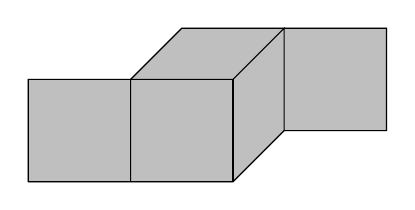
\begin{tikzpicture}[scale=1.3]
			\draw[fill,color=lightgray] (0,0) -- (1,0) -- (2,0) -- (2.5,0.5) -- (3.5,0.5) -- (3.5,1.5) -- (2.5,1.5) -- (1.5,1.5) -- (1,1) -- (0,1) -- (0,0);
			\draw (0,0) -- (1,0) -- (2,0) -- (2.5,0.5) -- (3.5,0.5) -- (3.5,1.5) -- (2.5,1.5) -- (1.5,1.5) -- (1,1) -- (0,1) -- (0,0);
			\draw (1,0) -- (1,1) -- (2,1) -- (2.5,1.5) -- (2.5,0.5);
			\draw (2,0) -- (2,1);
			\end{tikzpicture} \hspace{2cm}
			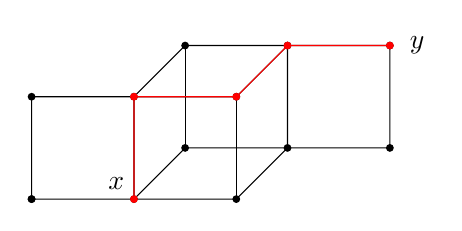
\begin{tikzpicture}[scale=1.3]
			\draw (0,0) node[fill,circle,inner sep=1pt]{} -- (1,0) node[fill,circle,inner sep=1pt]{} -- (2,0) node[fill,circle,inner sep=1pt]{} -- (2.5,0.5) node[fill,circle,inner sep=1pt]{} -- (3.5,0.5) node[fill,circle,inner sep=1pt]{} -- (3.5,1.5) node[fill,circle,inner sep=1pt]{} -- (2.5,1.5) node[fill,circle,inner sep=1pt]{} -- (1.5,1.5) node[fill,circle,inner sep=1pt]{} -- (1,1) node[fill,circle,inner sep=1pt]{} -- (0,1) node[fill,circle,inner sep=1pt]{} -- (0,0) node[fill,circle,inner sep=1pt]{};
			\draw (1,0) -- (1,1) -- (2,1) node[fill,circle,inner sep=1pt]{} -- (2.5,1.5) -- (2.5,0.5) -- (1.5,0.5) node[fill,circle,inner sep=1pt]{} -- (1,0);
			\draw (2,0) -- (2,1) ;
			\draw (1.5,0.5) -- (1.5,1.5);
			
			\draw[color=red] (1,0) node[fill,circle,inner sep=1pt]{} -- (1,1) node[fill,circle,inner sep=1pt]{} -- (2,1) node[fill,circle,inner sep=1pt]{} -- (2.5,1.5) node[fill,circle,inner sep=1pt]{} -- (3.5,1.5) node[fill,circle,inner sep=1pt]{};
			
			\draw (1,0) node[anchor=south east] {$x$};
			\draw (3.6,1.5) node[right] {$y$};
			\end{tikzpicture}
			\caption{Ein kubischer Komplex und sein $1$-Skelett. Es gilt $D(x,y) = 4$.} 
		\end{figure}
\end{beispiel}

\begin{lemma}
	\label{lemma:3.21}
		Sei $X$ ein $\CAT$ kubischer Komplex.
		Dann gilt für alle $x,y \in X^{(0)}$:
		\[
			D(x,y) = \# \{ H \subseteq X : H \text{ ist Hyperebene in } X\text{ die } x \text{ und } y \text{ trennt}\}.
		\]
		
		\begin{figure}[h]
			\centering
			\begin{tikzpicture}[scale=2,>=Latex]
			
				\draw [very thick,blue,schraffiert=blue] (1,1.5) -- (2,1.5) -- (2.5,2) -- (1.5,2) -- cycle;
				\draw [very thick,teal,schraffiert=teal] (1.25,1.25) -- (2.25,1.25) node[anchor=north west]{$H_3$} -- (2.25,2.25) -- (1.25,2.25) -- cycle;
				\draw [very thick,orange,schraffiert=orange] (1.5,1) -- (2,1.5) -- (2,2.5) -- (1.5,2) -- cycle;
				\draw [thick,dashed] (1,1) -- (1.5,1.5) -- (1.5,2.5);
				\draw [thick,dashed] (1.5,1.5) -- (2.5,1.5);
				\draw (0,1) -- (2,1) -- (2,0) -- (1,0) -- (1,2) -- (1.5,2.5) -- (3.5,2.5) -- (3.5,1.5) -- (2.5,1.5) -- (2,1) -- (2,2) -- (2.5,2.5);
				\draw (0,1) -- (0,2) -- (2,2);
				\draw (2.5,1.5) -- (2.5,2.5);
				
				\draw [color=red] (1,1) node[fill,circle,inner sep=1.5pt]{};
				\draw [color=red] (3.5,2.5) node[fill,circle,inner sep=1.5pt]{};
				\draw [color=red] (1,1) node[anchor=north east]{$x$};
				\draw [color=red] (3.5,2.5) node[right]{$y$};
				
				\draw [very thick,blue] (0,1.5) node[left]{$H_1$} -- (1,1.5);
				\draw [very thick,orange] (1.5,0) node[below]{$H_2$} -- (1.5,1);
				\draw [very thick,blue] (2.5,2) -- (3.5,2);
				\draw [very thick,red] (1,1) -- (1,2) -- (2,2) -- (2.5,2.5) -- (3.5,2.5);
				
				\draw [very thick,Magenta3] (3,1.5) node[below]{$H_4$} -- (3,2.5);
				\draw [color=red] (2.5,0.5) node[right]{$D(x,y) = 4$};
			\end{tikzpicture}
		\end{figure}
\end{lemma}
\newpage
\begin{definition}[medianer Graph]
	\label{def:3.22}
		Sei $\Gamma = (V,E)$ ein Graph.
		Das Intervall $I(u,v)$ für $u,v \in V$ ist definiert durch 
		\[
			I(u,v) = \{x \in V : d(u,v) = d(u,x) + d(x,v)\}
		\]
		Ein Graph $\Gamma$ heißt \Index{median}, falls für $u,v,w \in V$ paarweise verschieden gilt:
		\[
			\#(I(u,v) \cap I(u,w) \cap I(v,w)) = 1.
		\]
\end{definition}

\begin{beispiel}
	\label{bsp:3.23}
	\mbox{} \\[-1.3cm]
	\begin{figure}[h]
		\centering
		\begin{tikzpicture}[scale=1,>=Latex]
			\foreach \x in {2,...,5}{
				\draw (\x,1.5) -- (\x,5.5);
				\draw (1.5,\x) -- (5.5,\x);
			}
			\foreach \y in {1.96,2.96,3.96,4.96}
				\foreach \x in {1.96,2.96,3.96}
					\draw [color=red] (\x,\y) node [fill,circle,inner sep=2pt]{};
					
			\foreach \y in {3.96,4.96}
				\foreach \x in {2.04,3.04,4.04,5.04}
					\draw [color=blue] (\x,\y) node [fill,circle,inner sep=2pt]{};		

			\foreach \y in {2.04,3.04,4.04}
				\foreach \x in {4,5}
					\draw [color=Green4] (\x,\y) node [fill,circle,inner sep=2pt]{};	
					
			\draw [color=Magenta3] (1.95,5.05) node[anchor=south east]{$u$};
			\draw [color=Magenta3] (5.05,4.05) node[anchor=south west]{$w$};
			\draw [color=Magenta3] (4.05,1.95) node[anchor=north west]{$v$};
			
			\draw [thick,color=Magenta3] (4,4) circle (.35);
			
			\draw [color=red] (2,2) node[anchor=north east]{$I(u,v)$};
			\draw [color=blue] (5,5) node[anchor=south west]{$I(u,w)$};
			\draw [color=Green4] (5,2) node[anchor=north west]{$I(v,w)$};
			
			\draw [color=Magenta3] (7,3) node[right]{$I(u,v) \cap I(v,w) \cap I(u,w)$};
			\draw [very thick,dashed,Magenta3] (4.3,3.7) -- (6.8,3);
		\end{tikzpicture}

	\end{figure}
\end{beispiel}

\begin{satz}
	\label{satz:3.24}
		Sei $X$ ein $\CAT$ kubischer Komplex und $X^{(1)}$ das $1$-Skelett.
		Dann ist $(X^{(1)},D)$ median.
\end{satz}

\begin{beweis}
	Wir benötigen folgendes Hilfslemma:
	
	Seie $x,y \in X^{(0)}$ beliebig.
	Dann gilt:
	\[
		z \in I(x,y) \Leftrightarrow \text{ es existiert keine Hyperebene, die } z \text{ und } \{x,y\} \text{ trennt.}
	\]
	
	\textit{Beweis des Hilfslemmas:}
	Wir definieren
	\[
		W(x,y) := \{H \subseteq X : H \text{ ist Hyperebene, die } x \text{ und } y \text{ trennt.}\}
	\]
	Nach \autoref{lemma:3.21} gilt $D(x,y) = \#W(x,y)$.
	Wir erhalten
	\begin{align*}
		z \in I(x,y) &\stack{\text{Def.}}{\Leftrightarrow} D(x,y) = D(x,z) + D(z,y) \\
		&\stack{\ref{lemma:3.21}}{\Leftrightarrow} \#W(x,y) = \#W(x,z) + \#W(z,y) \\
		&\stack{}{\Leftrightarrow} W(x,y) = W(x,z) \sqcup W(z,y) \\
		&\stack{}{\Leftrightarrow} \text{ es existiert keine Hyperebene, die } z \text{ und } x \text{ trennt und } z \text{ und } y \text{ trennt} \\
		&\stack{}{\Leftrightarrow} \text{ es existiert keine Hyperebene, die } z \text{ und } \{x,y\} \text{ trennt}
	\end{align*}
	
	Zurück zum eigentlichen Beweis:
	Seien $x,y,z \in X^{(0)}$ paarweise verschieden.
	\begin{enumerate}[(i)]
		\item Zuerst zeigen wir $I(x,y) \cap I(x,z) \cap I(y,z) \neq \emptyset$.
		Wähle $m \in I(x,y) \cap I(x,z)$ mit $D(x,m)$ maximal.
		Zu zeigen ist $m \in I(y,z)$.
		
		\begin{minipage}{0.75\textwidth}
			Angenommen, $m \notin I(y,z)$.
			Nach dem Hilfslemma existiert eine Hyperebene $H$, die $m$ und $\{y,z\}$ trennt.
			Wähle $H$ mit minimalem Abstand zu $m$.
			
			Wähle $w \in H^+$ mit $D(m,w) = 1$.
			Es gilt $w \in I(x,y)$ und $w \in I(x,z)$.
			Weiter gilt $D(x,w) = D(x,m) + D(m,w) \geq D(x,m)$.
			Dies ist ein Widerspruch, da $m$ mit maximalem Abstand gewählt wurde.
		\end{minipage}
		~
		\begin{minipage}{0.2\textwidth}
			\begin{flushright}
				\begin{tikzpicture}[scale=1,>=Latex]
				\draw (0,.7) -- (0,3.75) node[above]{$H$};
				\draw (-.5,3.5) node[left]{$H^-$};
				\draw (.5,3.5) node[right]{$H^+$};
				
				\draw [thick] (-.5,2) node[below]{$m$} -- (.5,2) node[below]{$w$};
				\draw (-.5,2) node[fill,circle,inner sep=1.5pt]{};
				\draw (.5,2) node[fill,circle,inner sep=1.5pt]{};
				
				\draw (1,3) node[fill,circle,inner sep=1.5pt]{};
				\draw (1,3) node[right]{$y$};
				\draw (1,1) node[fill,circle,inner sep=1.5pt]{};
				\draw (1,1) node[right]{$z$};
			\end{tikzpicture}
			\end{flushright}
		\end{minipage}
		
		Es ist $w \in I(x,y)$:
		Ansonsten existiert nach Hilfslemma eine Hyperebene $J$, die $w$ und $\{x,y\}$ trennt.
		Es gilt $m \notin J^+$, denn $m \in I(x,y)$, also $m \in J^-$.
		Folglich trennt die Hyperebene $J$ $w$ und $m$.
		Es gilt $D(m,w) = 1$, das heißt $J = H$, aber $H$ trennt $m$ und $y$. Widerspruch.
		
		\item Zur Eindeutigkeit:
		Wir definieren
		\[
			\mathcal{HR} := \{\text{Halbräume, die mindestens zwei Elemente aus } x,y,z \text{ enthalten}\}.
		\]
		Es gilt $I(x,y) \subseteq \cap \{\text{Halbräume, die } x \text{ und } y \text{ enthalten}\}$.
		\[
			I(x,y) \cap I(x,z) \cap I(y,z) \subseteq \cap \mathcal{HR}
		\]
		Angenommen, es existieren $m_1,m_2 \in I(x,y) \cap I(x,z) \cap I(y,z)$ mit $m_1 \neq m_2$.
		Da $m_1 \neq m_2$, ist $D(m_1,m_2) = \#W(m_1,m_2) > 0$.
		Es existiert also eine Hyperebene $H$, die $m_1$ und $m_2$ trennt.
		O.B.d.A. seien $x,y \in H^-$.
		Dann folgt $H^- \in \mathcal{HR}$, aber $H^+ \notin \mathcal{HR}$.
		Da $I(x,y) \cap I(x,z) \cap I(y,z) \subseteq \cap \mathcal{HR}$, ist $m_2 \notin \cap \mathcal{HR}$, also auch $m_2 \notin I(x,y) \cap I(x,z) \cap(y,z)$.
		Widerspruch. \qedhere
	\end{enumerate}
\end{beweis}
\newpage
\begin{beweis}[\autoref{thm:3.14}]
	Wir zeigen per Induktion, dass für $k = 2, \dots, m$ die $k$-elementigen Mengen aus $\mathcal{S}$ sich nichttrivial schneiden.
	Für $k=2$ ist dies nach Voraussetzung erfüllt.
	Wir definieren $Y := X_3 \cap X_4 \cap \dots \cap X_k$.
	Wir wissen: $X_1 \cap  X_2 \neq \emptyset, X_1 \cap Y \neq \emptyset$ und $X_2 \cap Y \neq \emptyset$ nach Induktionsannahme.
	
	Nun sind $Y, X_1 \cap X_2, X_1 \cap Y$ und $X_2 \cap Y$ konvexe, also insbesondere $\CAT$ kubische Unterkomplexe.
	Wähle Ecken $p \in X_1 \cap Y$, $q \in X_2 \cap Y$ und $r \in X_1 \cap X_2$.
	Da $Y$ ein $\CAT$ kubischer Unterkomplex ist und $p,q \in Y$, liegt auch $I(p,q) \subseteq Y$.
	Ebenso ist $p,r \in X_1$, also $I(p,r) \subseteq X_1$ und $q,r \in X_2$, also $I(q,r) \subseteq X_2$.
	Weiter ist $I(p,q) \cap I(p,r) \cap I(q,r) = \{m(p,q,r)\}$ und $m(p,q,r) \in Y$.
	Folglich ist $m(p,q,r) \in X_1 \cap X_2 \cap Y$. \qedhere
\end{beweis}

\begin{satz}
	\label{satz:3.25}
	Sei $G := \sprod{g_1,\dots,g_k}$ eine endlich erzeugte Gruppe und $X$ ein $\CAT$ kubischer Komplex. \marginnote{03.02. \\ \ [19]}
	Sei weiter $\Phi \colon G \rightarrow \Isom(X)$ eine isometrische Wirkung.
	Wenn $\Fix_\Phi(\sprod{g_i})$ kubische Unterkomplexe sind und $\Fix_\Phi(\sprod{g_i}) \cap \Fix_\Phi(\sprod{g_j}) \neq \emptyset$ für $i,j = 1, \dots, k$, dann ist $\Fix_\Phi(G) \neq \emptyset$.
\end{satz}

\begin{beweis}
	\autoref{thm:3.14} mit $\mathcal{S} := \{\Fix_\Phi(\sprod{g_1}),\dots,\Fix_\Phi(\sprod{g_k})\}$. \qedhere
\end{beweis}

\begin{minipage}{.6\textwidth}
	\begin{no-bem}
		Im Allgemeinen ist $\Fix_\Phi(\sprod{g_i})$ kein kubischer Unterkomplex:
		
		Sei $G:= \ZZ \diagup 2\ZZ$ und $X := \RR^2$ und definiere die Wirkung
		\begin{align*}
		\Phi\colon G &\longrightarrow \Isom(X) \\
		\ol{0} &\longmapsto \id_{\RR^2} \\
		\ol{1} &\longmapsto \begin{pmatrix}
		0 & 1 \\
		1 & 0
		\end{pmatrix}
		\end{align*}
	\end{no-bem}
\end{minipage} \hfill
\begin{minipage}{.37\textwidth}
	\centering
	\begin{tikzpicture}[scale=.66,>=Latex]
	\foreach \x in {1,...,5} {
		\draw (\x,0) -- (\x,6);
		\draw (0,\x) -- (6,\x);
	}
	\draw [color=red,very thick] (.5,.5) -- (5.5,5.5) node[right]{$\Fix_\Phi(\sprod{\ol{1}})$};
	\draw (3,3) node[fill,circle,inner sep=1.5pt]{};
	\draw (3,3) node[anchor=north west]{$0$};
	\end{tikzpicture}
\end{minipage}

\begin{theorem}[\textsc{Helly}s Theorem für $\CAT$-Räume]
	\label{thm:3.26}
	Sei $X$ ein $d$-dimensionaler (Überdeckungsdimension) vollständiger $\CAT$-Raum und $\mathcal{S}$ eine endliche Familie von (nichtleeren) konvexen abgeschlossenen Teilmengen.
	Wenn sich jeweils $(d+1)$ Elemente aus $\mathcal{S}$ nichttrivial schneiden, dann ist $\cap \mathcal{S} \neq \emptyset$.
\end{theorem}

\section{\textsc{Gromov}s Link-Bedingung}
\label{sec:3.2}
	\textbf{Leitfrage:} Wie kann man in kubischen Komplexen die lokale $\CAT$ Eigenschaft nachprüfen?
	
	Ab jetzt sei $X$ ein endlich dimensionaler kubischer Komplex.
	
\begin{definition}[Simplizialkomplex]
	\label{def:3.27}
	Sei $Y$ eine Menge und $\Delta \subseteq \pot(Y)$ eine Menge von endlichen Teilmengen aus $Y$.
	Wir nennen $(\Delta,\subseteq)$ einen \Index{Simplizialkomplex}, wenn gilt:
	\[
		a \subseteq b \in \Delta \quad \Rightarrow \quad a \in \Delta,
	\]
	das heißt $\Delta$ ist abgeschlossen bezüglich Abstieg.
	
	Die Elemente aus $\Delta$ heißen \textbf{Simplizes}.
	Die Dimension eines Simplex $a \in \Delta$ ist $k$, falls $\# a = k+1$.
	Wir setzen $\Delta^{(k)} = \{a \in \Delta : \dim(a) = k\}$.
\end{definition}

\begin{beispiel}
	\label{bsp:3.28}
	$Y := \NN, \Delta= \{\emptyset,\{1\},\{2\},\{3\},\{4\},\{1,2\},\{1,3\},\{2,3\},\{1,2,3\}\}$
	\begin{figure}[h]
		\centering
		\begin{tikzpicture}[scale=1.5,>=Latex]
			\coordinate (A) at (0,0);
			\coordinate (B) at (1,0);
			\coordinate (C) at (1,1);
			\coordinate (D) at (0,1);
			
			\draw [color=teal,schraffiert=teal] (B) -- (C) -- (D) -- cycle;
			\draw [color=RoyalBlue4,ultra thick] (B) -- (C) -- (D) -- cycle;
			\foreach \x in {A,B,C,D}
				\draw [color=red] (\x) node[fill,circle,inner sep=2pt]{};
				
			\draw (A) node[anchor=north east]{$4$};
			\draw (B) node[anchor=north west]{$3$};
			\draw (C) node[anchor=south west]{$2$};
			\draw (D) node[anchor=south east]{$1$};
		\end{tikzpicture}
	\end{figure}
\end{beispiel}

\begin{definition}[Fahnenkomplex]
	\label{def:3.29}
	Ein Simplizialkomplex $\Delta \subseteq \pot(Y)$ heißt \Index{Fahnenkomplex}, wenn folgendes gilt:
	
	Sei $a \subseteq Y$ eine Teilmenge.
	Wenn alle zweielementigen Teilmengen aus $a$ in $\Delta$ liegen, dann liegt $a \in \Delta$.
\end{definition}

In Worten ausgedrückt bedeutet dies:
Wenn der Rand eines Simplex in $\Delta$ liegt, dann muss auch schon das gesamte Simplex in $\Delta$ liegen.
Der Simplizialkomplex aus \autoref{bsp:3.28} ist beispielsweise ein Fahnenkomplex.
Der Simplizialkomplex definiert durch $Y:=\NN$, $\Delta = \{\emptyset,\{1\},\{2\},\{3\},\{1,2\},\{1,3\},\{2,3\}\}$ ist jedoch kein Fahnenkomplex:
lle zweielementigen Teilmengen von $\{1,2,3\}$ sind in $\Delta$ enthalten, jedoch nicht $\{1,2,3\}$ selbst.
 
\begin{definition}
	\label{def:3.30}
	Sei $x \in X$ eine Ecke.
	Sei $\varepsilon = \frac{1}{2}$.
	Die kubische Struktur von $X$ induziert auf $\partial B_\varepsilon(x)$ eine simpliziale Struktur wie folgt:
	
	Setze die Menge der $0$-Simplizes als $\partial B_\varepsilon(x) \cap k$, $k \subseteq X$ ist Seite eines Würfels und isometrisch zu $[0,1]$.
	Nun:
	\[
		\{\Underbrace{x_1,\dots,x_{k+1}}{\mathclap{\text{0-Simplizes und paarw. versch.}}}\} \text{ ist } k \text{-Simplex} \quad \Leftrightarrow \quad \text{es ex. Würfel } W \subseteq X \text{ mit } \dim(W) = k+1 \text{ und } \{x_1,\dots,x_{k+1}\} \subseteq W
	\]
	Dieser Simplizialkomplex heißt der \Index{Link} bzw. \textbf{Eckenlink} von $x$ in $X$.
\end{definition}

\begin{beispiel}
	\label{bsp:3.31}
	\mbox{} \\[-1.5cm]
	\begin{enumerate}[(i)]
		\item \mbox{} \\[-1cm]
		\begin{figure}[h]
			\centering
			$\vcenter{\hbox{\begin{tikzpicture}[scale=1,>=Latex]
				\foreach \x in {2,...,4} {
					\draw (\x,1) -- (\x,5);
					\draw (1,\x) -- (5,\x);
				}
				\draw (3,3) node[fill,circle,inner sep=1.5pt]{};
				\draw (3,3) node[anchor=north west]{$x$};
				\draw [color=red,thick] (3,3) circle (.6);
			\end{tikzpicture}}} \hspace{3cm}
			\vcenter{\hbox{\begin{tikzpicture}[scale=1.5,>=Latex]
			\foreach \x in {2,...,4} {
				\draw (\x,1.9) -- (\x,4.1);
				\draw (1.9,\x) -- (4.1,\x);
			}
			\draw (3,3) node[fill,circle,inner sep=1.5pt]{};
			\draw (3,3) node[anchor=north west]{$x$};
			\draw [color=red, very thick]
				(2.5,3) node[fill,circle,inner sep=1.5pt]{} --
				(3,2.5) node[fill,circle,inner sep=1.5pt]{} --
				(3.5,3) node[fill,circle,inner sep=1.5pt]{} --
				(3,3.5) node[fill,circle,inner sep=1.5pt]{} -- cycle;
			\draw [color=red] (3.3,3.3) node[right]{$\operatorname{Lk}(x)$};
			\end{tikzpicture}}}$		
		\end{figure} \newpage
		\item \mbox{} \\[-1cm]
		\begin{figure}[h]
			\centering
			$\vcenter{\hbox{\begin{tikzpicture}[scale=2,>=Latex]
				\draw [schraffiert3=teal] (0,0) -- (-.75,-.5) -- (0,-1) -- (.75,-.5) -- cycle;
				\draw [schraffiert2=teal] (0,0) -- (-.75,-.5) -- (-.75,.5) -- (0,1) -- cycle;
				\draw [schraffiert=teal] (0,0) -- (0,1) -- (.75,.5) -- (.75,-.5) -- cycle;
				\draw [color=red,thick] (0,.5) to[out=210,in=90] (-.375,-.25);
				\draw [color=red,thick] (0,.5) to[out=-30,in=90] (.375,-.25);
				\draw [color=red,thick] (-.375,-.25) to[out=-45,in=225] (.375,-.25);
				\draw (0,0) node[fill,circle,inner sep=1.5pt]{};
				\draw (0,0) node[below]{$x$};
			\end{tikzpicture}}} \hspace{2cm}
			\vcenter{\hbox{\begin{tikzpicture}[scale=2.5,>=Latex]
				\draw (0,0) -- (0,.7);
				\draw (0,0) -- (.525,-.35);
				\draw (0,0) -- (-.525,-.35);
				\draw (0,0) node[fill,circle,inner sep=1.5pt]{};
				\draw (0,0) node[below]{$x$};
				\draw [color=red,very thick]
					(0,.5) node[fill,circle,inner sep=1.5pt]{} --
					(-.375,-.25) node[fill,circle,inner sep=1.5pt]{} --
					(.375,-.25) node[fill,circle,inner sep=1.5pt]{} -- cycle;
				\draw [color=red] (.2,.4) node[right]{$\operatorname{Lk}(x)$};
			\end{tikzpicture}}}$
		\end{figure}
	\end{enumerate}
\end{beispiel}

\begin{theorem}[\textsc{Gromov}s Link-Bedingung]
	\label{thm:3.32}
	Sei $X$ ein endlich dimensionaler kubischer Komplex.
	$X$ ist genau dann lokal $\CAT$, wenn alle seine Eckenlinks Fahnenkomplexe sind.
\end{theorem}

\begin{figure}[h]
	\centering
	\begin{tikzpicture}[scale=2,>=Latex]
		\draw [dashed] (1,1) -- (1.5,1.5) -- (2.5,1.5);
		\draw [dashed] (1.5,1.5) -- (1.5,2.5);
	
		\draw [color=DodgerBlue3,very thick]
			(0,1.5) -- (.5,2);
		
		\draw [color=Chocolate3,very thick]
			(0,1.5) -- (.5,1);
			
		\draw [color=DeepPink3,very thick]
			(.5,1) -- (1,1.5);
		\draw [color=DeepPink3,very thick,schraffiert3=DeepPink3]
			(1,1.5) -- (1.3,1.3) -- (1.5,1) -- cycle;
		\draw [color=DeepPink3,very thick]
			(1.5,1) -- (1,.5);
			
		\draw [color=Green3,very thick]
			(.5,2) -- (1,1.5);
					
		\draw [color=Green3,very thick,schraffiert=Green3]
			(1,1.5) -- (1.5,2) -- (1.25,2.25) -- cycle;
			
		\draw [color=Firebrick3,very thick,schraffiert=Firebrick3]
			(1.25,2.25) -- (1.5,2.02) -- (2,2.5) --	cycle;
		
		\draw [color=Gold2,very thick,schraffiert=Gold2]
			(1.5,2) -- (1.95,1.5) -- (1.32,1.32) -- cycle;
		
		\draw [color=DeepSkyBlue1,very thick,schraffiert3=DeepSkyBlue1]
			(2,2.5) -- (2.2,2.2) -- (2.5,2) -- cycle;
		\draw [color=DeepSkyBlue1,very thick]
			(2.5,2) -- (3,2.5);
		
		\draw [color=Orchid2,very thick,schraffiert=Orchid2]
			(2.5,2) -- (2,1.5) -- (2.25,1.25) -- cycle;
		\draw [color=Orchid2,very thick]
			(2.5,2) -- (3,1.5);
		
		\draw [color=RoyalBlue3,very thick, schraffiert=RoyalBlue3]
			(1.5,2) -- (2.2,2.2) -- (2,1.5) -- cycle;
		\draw [color=RoyalBlue3] (2,2) node[fill,circle,inner sep=1.5pt]{};
		
		\draw [color=Purple3,very thick, schraffiert2=Purple3]
			(1.5,1) -- (2,1.5) -- (2.25,1.25) -- cycle;
		\draw [color=Purple3,very thick]
			(1.5,1) -- (2,.5);
		
		\draw [color=SkyBlue1,very thick]
			(1,.5) -- (1.5,0);
		
		\draw [color=Orange1,very thick]
			(1.5,0) -- (2,.5);
		
		\draw [color=Ivory4,very thick]
			(3,1.5) -- (3.5,2);
		
		\draw [color=DeepPink1,very thick]
			(3.5,2) -- (3,2.5);
		
		\draw [thick] (0,1) -- (2,1) -- (2,0) -- (1,0) -- (1,2) -- (1.5,2.5) -- (3.5,2.5) -- (3.5,1.5) -- (2.5,1.5) -- (2,1) -- (2,2) -- (2.5,2.5);
		\draw [thick] (0,1) -- (0,2) -- (2,2);
		\draw [thick] (2.5,1.5) -- (2.5,2.5);

		\draw [color=DeepPink1] (3.5,2.5) node[fill,circle,inner sep=1.5pt]{};
		\draw [color=Ivory4] (3.5,1.5) node[fill,circle,inner sep=1.5pt]{};
		\draw [color=Orange1] (2,0) node[fill,circle,inner sep=1.5pt]{};
		\draw [color=SkyBlue1] (1,0) node[fill,circle,inner sep=1.5pt]{};
		\draw [color=Purple3] (2,1) node[fill,circle,inner sep=1.5pt]{};
		\draw [color=Orchid2] (2.5,1.5) node[fill,circle,inner sep=1.5pt]{};
		\draw [color=DeepSkyBlue1] (2.5,2.5) node[fill,circle,inner sep=1.5pt]{};
		\draw [color=Gold2] (1.5,1.5) node[fill,circle,inner sep=1.5pt]{};
		\draw [color=Firebrick3] (1.5,2.5) node[fill,circle,inner sep=1.5pt]{};
		\draw [color=Green3] (1,2) node[fill,circle,inner sep=1.5pt]{};
		\draw [color=DeepPink3] (1,1)  node[fill,circle,inner sep=1.5pt]{};
		\draw [color=DodgerBlue3] (0,2) node[fill,circle,inner sep=1.5pt]{};
		\draw [color=Chocolate3] (0,1) node[fill,circle,inner sep=1.5pt]{};	
	\end{tikzpicture}
	\caption{Dieser kubische Komplex ist lokal $\CAT$, da alle seine Links Fahnenkomplexe sind.}
\end{figure}

\newpage

\section*{Zusammenfassung}
\begin{itemize}
	\item $\CAT$-Räume
		\begin{itemize}
			\item eindeutig geodätisch
			\item kontrahierbar
			\item einfach zusammenhängend
			\item Vervollständigung ist ebenfalls $\CAT$
		\end{itemize}
	\item Beispiele für $\CAT$-Räume
		\begin{itemize}
			\item $(V,\Norm{\cdot})$ ist $\CAT \Leftrightarrow (V,\Norm{})$ ist ein Prähilbertraum
			\item konvexe Teilmengen von $\CAT$-Räumen
			\item simpliziale Bäume
		\end{itemize}
	\item Satz von \textsc{Cartan-Hadamard}
		\begin{itemize}
			\item Ist $X$ ein vollständiger zusammenhängender lokaler $\CAT$-Raum, dann ist seine universelle Überlagerung $\tilde{X}$ ebenfalls $\CAT$.
			\item $X$ ist genau dann vollständig, zusammenhängend, lokal $\CAT$ und einfach zusammenhängend, wenn $X$ ein vollständiger $\CAT$-Raum ist.
		\end{itemize}
	\item Wie kann man die lokale $\CAT$-Eigenschaft testen?
		\begin{itemize}
			\item Kubische Komplexe und \textsc{Gromov}s Link-Bedingung
		\end{itemize}
	\item Gruppenwirkungen auf $\CAT$-Räumen
		\begin{itemize}
			\item \textsc{Bruhat-Tits}-Fixpunktsatz:
			Jede Wirkung einer endlichen Gruppe auf einen vollständigen $\CAT$-Raum besitzt einen globalen Fixpunkt.
			\item \textsc{Helly}s Theorem für Bäume und kubische Komplexe sowie Anwendung auf Gruppenwirkungen
			\item \textsc{Helly}s Theorem für kubische Komplexe
			\item Eigenschaft $\prF{A}$
		\end{itemize}
\end{itemize}
